\documentclass{beamer}
\usepackage{beamerthemesplit}
\usetheme{SPbGU}
%{CambridgeUS}
% Выпишем часть возможных стилей, некоторые из них могут содержать
% дополнительные опции
% Darmstadt, Ilmenau, CambridgeUS, default, Bergen, Madrid, AnnArbor,Pittsburg, Rochester,
% Antiles, Montpellier, Berkley, Berlin
\usepackage{pdfpages}
\usepackage{amsmath}
\usepackage{cmap} % for serchable pdf's
\usepackage[T2A]{fontenc} 
\usepackage[utf8]{inputenc}
\usepackage[english,russian]{babel}
\usepackage{indentfirst}
\usepackage{amsmath}
\usepackage{tikz}
\usepackage{graphicx}

\usetikzlibrary{shapes,arrows}
% Если у вас есть логотип вашей кафедры, факультета или университета, то
% его можно включить в презентацию.

%\usefoottemplate{\vbox{}}%  \tinycolouredline{structure!25}% {\color{white}\textbf{\insertshortauthor\hfill% \insertshortinstitute}}% \tinycolouredline{structure}% {\color{white}\textbf{\insertshorttitle}\hfill}% }}

%\logo{
\includegraphics[width=1cm]{SPbGU_Logo.png}}

%[GLR-анализатор]
\title[]{Модульный генератор синтаксических анализаторов}
\institute[СПбГУ]{
Санкт-Петербургский государственный университет \\
Математико-Механический факультет \\
Кафедра системного программирования }
%[Я.А. Кириленко, К.А. Улитин]


\author[Я.А. Кириленко, К.А. Улитин]{ Константин Андреевич Улитин \\
  \and  
  {\bfseries Научный руководитель:} ст.преп. СПбГУ Я.А. Кириленко \\ 
}

\date{23 марта 2011г.}

\begin{document}
\sloppy
{

\begin{frame}
\begin{center}
{
\includegraphics[width=1cm]{SPbGU_Logo.png}}
\end{center}
%\frame{ 
\titlepage
%}
\end{frame}
}

\begin{frame}
	\transwipe[direction=90]
	\frametitle{Предметная область}
Характеристики парсер-генераторов
	\begin{itemize}
		\item Класс принимаемых языков и грамматик
		\item Разрешение неоднозначностей в грамматике
		\item Скорость работы сгенерированного парсера/транслятора
		\item Возможности языка описания грамматики	
		\item Простота отладки грамматики
		\item Целевой язык	
		\item ...
	\end{itemize}
\end{frame}


\begin{frame}
	\transwipe[direction=90]
	\frametitle{Классы анализаторов}
Алгоритм разбора
	\begin{itemize}
		\item LL(k или *) с рекурсивным спуском – более удобная отладка, медленнее работает
		\item LR(k), LALR – «съедает» леворекурсивные грамматики
		\item GLR – неоднозначные грамматики
	\end{itemize}
Язык описания грамматики
	\begin{itemize}
		\item EBNF(*,+,?)
		\item Правила-шаблоны
		\item Модульность грамматики
	\end{itemize}
\end{frame}

%	\begin{block}{Простые грамматики (DSL, конфигурационные файлы, собственный протокол передачи данных)}
%		\begin{itemize}
%			\item Выбор способа описания грамматики
%			\item Переиспользование наработок других инструментов
%			\item Удобная интеграция с разрабатываемым приложением
%		\end{itemize}
%	\end{block}
%	\begin{block}{Сложные грамматики/диалекты}
%		\begin{itemize}
%			\item Широкие возможности языка описания трансляции
%			\item Выбор алгоритма разбора
%		\end{itemize}
%	\end{block}

\begin{frame}
	\transwipe[direction=90]
	\frametitle{Задача}
Генератор синтаксических анализаторов для среды .NET
	\begin{itemize}
		\item Переиспользование наработок других инструментов
		\item Удобная интеграция с разрабатываемым приложением
		\item Широкие возможности языка описания трансляции
		\item Выбор алгоритма разбора
	\end{itemize}
\end{frame}


\begin{frame}
	\transwipe[direction=90]
	\frametitle{YaccConstructor}
\begin{center}
{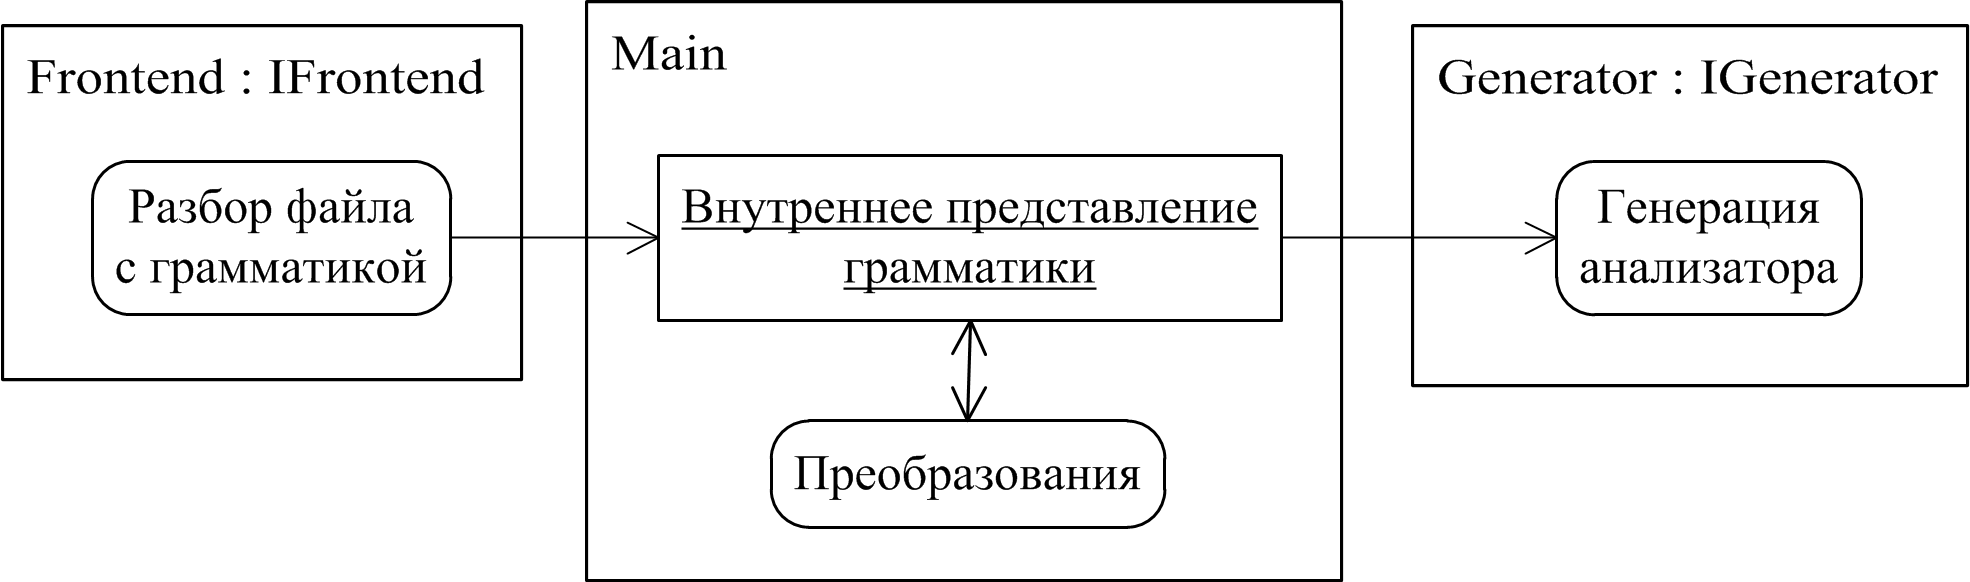
\includegraphics[scale=0.7]{arch.png}} %width=\textwidth
\end{center}
\end{frame}

\begin{frame}
	\transwipe[direction=90]
	\frametitle{Реализованные компоненты}
\begin{center}
{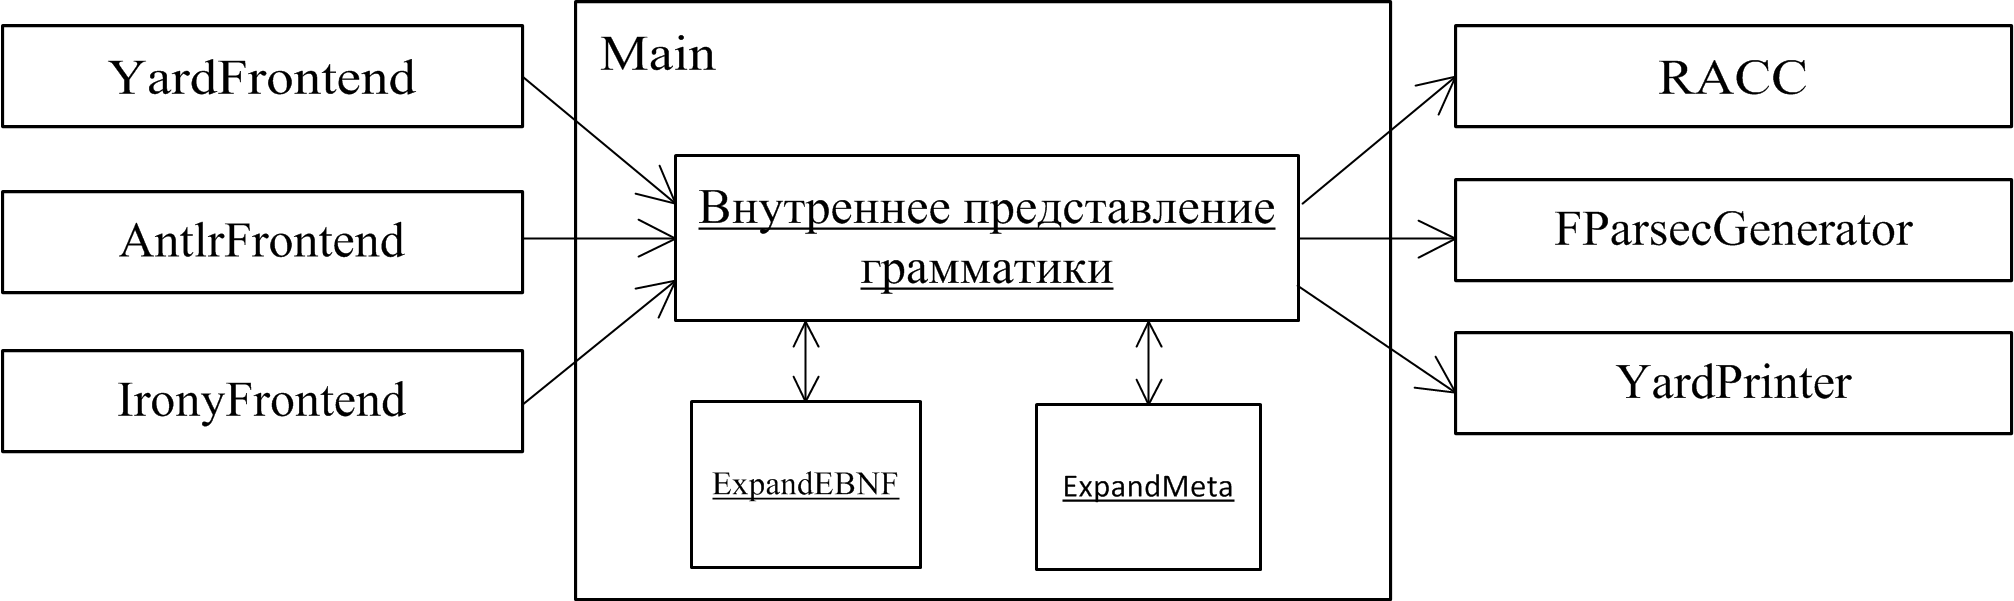
\includegraphics[scale=0.7]{components.png}}
\end{center}
\end{frame}

\begin{frame}
	\transwipe[direction=90]
	\frametitle{Особенности реализации}
	\begin{itemize}
		\item Command Line Interface
		\item Автозагрузка компонент
		\item Юнит-тестирование
	\end{itemize}
\end{frame}

\begin{frame}
	\transwipe[direction=90]
	\frametitle{Юзкейсы}
	\begin{enumerate}
		\item SQL.g \ensuremath{\rightarrow} \fbox{AntlrFrontend} \ensuremath{\rightarrow} \fbox{YardPrinter} \ensuremath{\rightarrow} SQL.yrd
		\item \fbox{YaccPrinter} перестал работать \\ Заменяем на \fbox{RACC} 
		\item Debug : \fbox{FParsecGenerator} \\Release : \fbox{RACC}
	\end{enumerate}
\end{frame}

\begin{frame}
	\transwipe[direction=90]
	\frametitle{Используемые технологии}
 При разработке используются следующие технологии
	\begin{itemize}
		\item Microsoft Visual Studio 2010, MSBuild
		\item F\#, FsLex, FsYacc
		\item NUnit
		\item SVN
	\end{itemize}	
Текущее состояние проекта\\
\href{http://code.google.com/p/recursive-ascent/}{http://code.google.com/p/recursive-ascent}
\end{frame}

\end{document}
